\section{Modeling An Election Algorithm as a Stationary Markov Chain}

%State how sequences are generated.
%State how transition probabilities are generated in the profile chain. State what the profile chain could be used for when collected.

% 3 sections
% Execution assumptions
% algorithmic changes
% producing the profile chain

\subsection{Execution Environment}

Execution occurs in a real-time partially synchronous environment.
Processes synchronize their clocks and execute steps of the election algorithm at predefined intervals.
Processes with clocks that are not sufficiently synchronized cannot form groups.
For this work, process execution occurs in an environment where the clocks are sufficiently synchronized to consistently form groups.

The execution environment is subject to omission failures.
In an omission failure, a message sent by one process to another process is lost in transit.
Omission failures can occur for many reasons.
Network congestion is a typical culprit.
Routers may drop packets or delay their delivery when there is a large amount of traffic or a network issue.
In a real-time environment, messages that are delayed and miss their real-time deadlines will have the same appearance as an omitted message.
Process delay can also cause a similar effect.
The execution environment for the election algorithm has a omission failure occurrence modeled as a Bernoulli trial.
In this model, each message has some probability $p$ of being delivered within the timing constraints imposed by the real-time schedule.
For the purpose of analyzing the effects of omission failures, processes are not subject to other faults.

\subsection{Election Algorithm}

A state machine for the election portion of the election algorithm is shown in Figure \ref{fig:statemachine}.
In the normal state, the election algorithm regularly searches for other coordinators to join with.
When another coordinator is identified, all other processes will yield to their future coordinator.
The method of selecting which process becomes the coordinator of the new group differentiates the invitation election algorithm from other approaches.
Regardless of the algorithm, the selection of the coordinator is always a race-condition and is difficult to model.

In the invitation election algorithm, processes are assigned a priority based on their process ID.
The coordinator with the highest priority is the first to send invites.
After a brief delay, if it appears that coordinator did not send their invites, the next highest process will send their invites.
Coordinators that receive invites will forward the invite to its group members.
Those processes will accept the invite.
Once a timeout expires, the coordinator will send a ``Ready'' message with a list of peers to all processes that accepted the invite.
The invited processes have timeouts for when they expect the ready message to arrive.
If the message does not arrive in time, the process will enter the recovery state where it resets to a group by itself.

\begin{figure*}[!t]
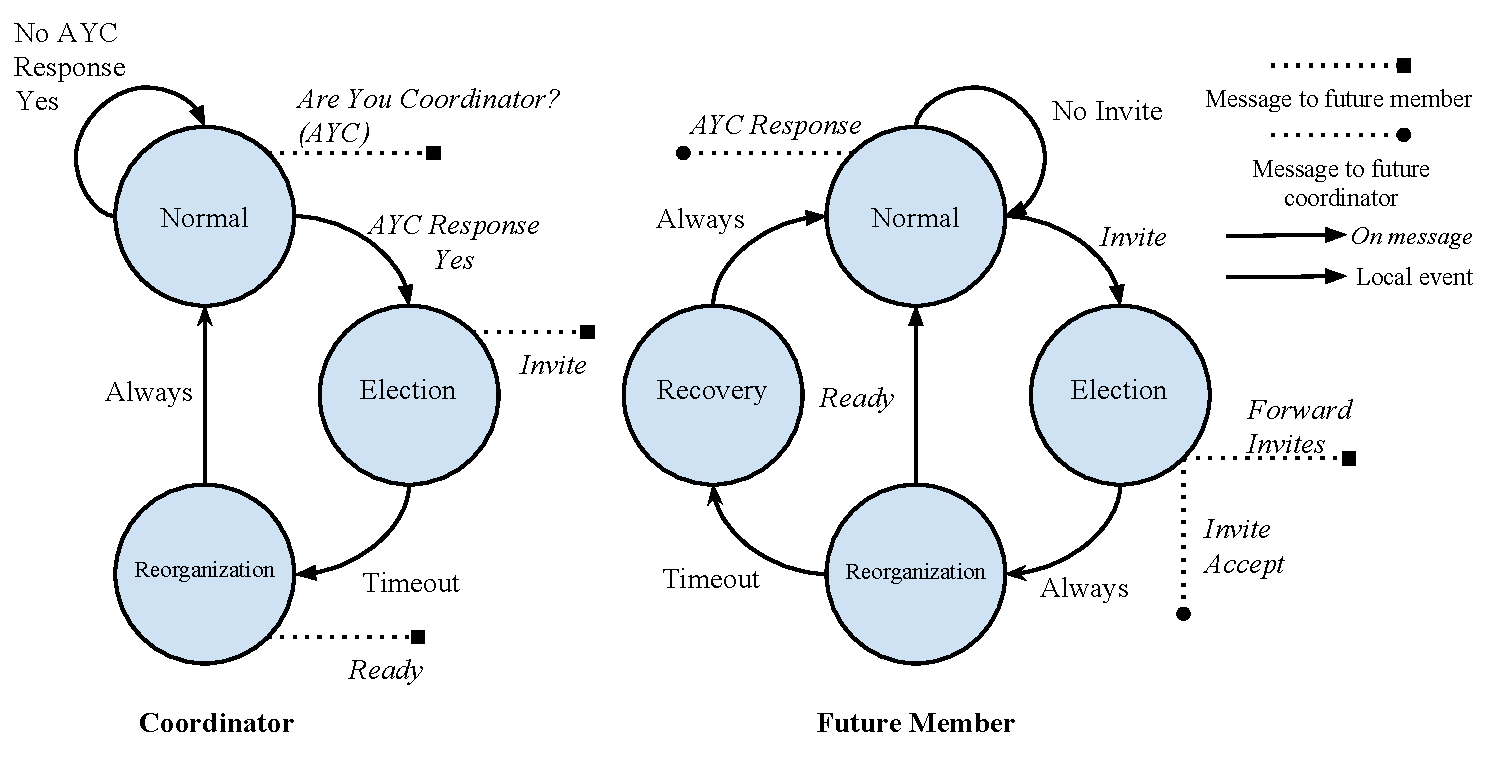
\includegraphics[width=\linewidth]{LeaderElectionStateDiagram.pdf}
\caption{State machine of a leader election. Processes start as coordinators in the ``Normal'' state and search for other coordinators to join with. Processes immediately respond to ``Are You Coordinator'' (AYC) messages they receive. The algorithm was modified by adding a ``Ready Acknowledgment'' message as the final step of completing the election. Additionally, processes only accept invites if they have received an ``AYC Response'' message from the inviting process.}
\label{fig:statemachine}
\end{figure*}

Once a group is formed it must be maintained.
To do this, processes occasionally exchange messages to verify the other is still reachable.
This interaction is shown in Figure \ref{fig:statemachine2}.
Coordinators send ``Are You Coordinator'' messages to members of its group to check if the process has left the group.
Group members send ``Are You There'' messages to the coordinator to verify they haven't been removed from the group, and to ensure the coordinator is still alive.
If processes fail to reply to received message before a timeout, they will leave the group.
Leaving the group can either be caused by the coordinator removing the process, or the process can enter a recovery state and leave the group, forming a new group by itself.

\begin{figure*}[!t]
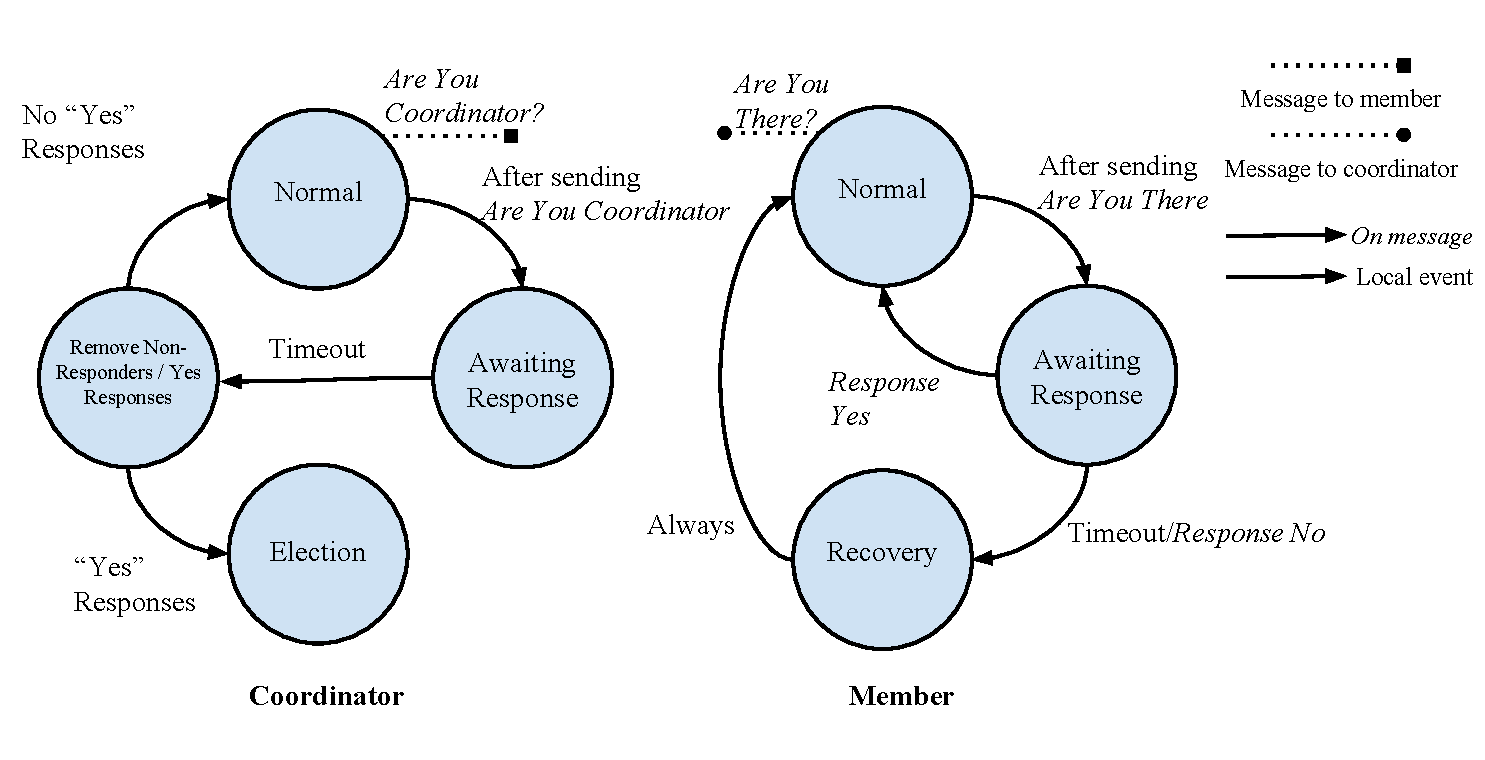
\includegraphics[width=\linewidth]{MaintainStateDiagram.pdf}
\caption{State machine of maintaining a group. The ``Are You Coordinator'' (AYC) messages are the same as those in Figure \ref{fig:statemachine}. AYC and ``Are You There'' (AYT) are periodically sent by processes, and responses to those messages are immediately sent by the receiving process. In the modified algorithm, the member does not enter the recovery state if they do not receive an AYT response before the timeout expires.}
\label{fig:statemachine2}
\end{figure*}

For a variety of reasons modeling this algorithm is very difficult.
In a distributed system information cannot be instantaneously spread throughout the system.
As a consequence, an omission failure will cause a process to miss out on information distributed by other processes.
In particular, an omission of a ``Ready'' message sent to group members cannot be known to the coordinator without an additional message.
This missing information normally causes the coordinator's observation of the group to be out-of-date.
If the observed state of the group is incorrect, it cannot be used in a Markov chain with perfect information.
When the coordinator's observation of the group is out-of-date, a state observed by the coordinator would conflict with one observed by a member.
In this case, the state observed the member is closer to the true state of the system.
This situation is not favorable to modeling the formation of groups.
This is true because, for the purpose managing the group, the observations of the coordinator are much more valuable than those of the members.

In the modified algorithm, members have uncertainty with respect to their membership, and the coordinator has perfect information about members that definitely are a part of the group.
The original ``Are You There'' approach for detecting failure (Figure \ref{fig:statemachine2}) also causes a similar effect.
Additionally, the election algorithm has an inherent race condition as part of its normal operation.
This race condition can make the selection of the group leader inconsistent: the highest priority process may not always win the election.
For the purpose of analyzing the system, having a consistent leader is important for capturing a consistent view of grouping.
Additionally, the resulting leader of a normal election is difficult to model since it would necessitate capturing a race-condition in the model.

In this work, we model what a process will observe as a result of omission failure.
Therefore, it is important a process's observations hold to the Markov property.
The original Garcia-Molina algorithm has been modified so the observations of the coordinator process have the Markov property.
The full modified algorithm is presented in Appendix \ref{apdx:algorithm}.
The following sections state the portions of the algorithm where the observation of the leader process does not yield the probability of next transition.
Changes to the algorithm relieved race conditions when selecting a leader, and made the state of the members a certainty for the coordinator.

\subsection{Leader Selection}

To alleviate the inherit race condition of leader selection, without loss of generality, a fixed leader process was selected.
This process was the only one that could become the leader of a multiprocess group.
This is shown in Figure \ref{fig:statemachine}, where only the selected process can send invite messages.
This simplification was applied because the configuration of the system with a larger number of processes depended on the configuration of the other processes.
Without this simplification, the state of the rest of the system would not have the memoryless property.
The state of the processes that are not in the observers group would change each round.
As a consequence the state of the rest of the system and the likelihood of forming a specific group size would change each step if other processes could become leader.
A probabilistic prediction would depend on how long the processes have been separated.
After a long enough period of time the distribution of states for the processes could be found using a steady-state analysis.
However, when processes enters the ``Recovery'' state they are deterministically placed in the alone state.
As a consequence the state of the system depends on the number of steps since the last reconfiguration, which violates the memoryless property.

Suppose P1 fails to detect P2 and P3 multiple times.
The probability P2 has grouped with P3 could then be modeled as a two process sub-case of this three process case.
Let this two process sub-case be described with a profile chain $P_{sub}$.
The probability of P2 and P3 joining P1's group depends on the state of the sub-case.
Additionally the probability distribution of an observation of the sub-case depends how many steps the sub-case has completed.
If $P_{sub}$ is ergodic, then $Steady(P_{sub}{}) \neq [1.0 \quad 0]$.
Each step of the sub-case ($n$) will move its distribution asymptotically closer to the steady-state:

\begin{equation} [1.0 \quad 0] * \lim_{n \to \infty}P_{sub}^n = Steady(P_{sub}) \end{equation}

Since the initial state of the algorithm in the sub-case must be un-grouped ($[1.0 \quad 0]$), and the process is ergodic, the probability distribution of the sub-case depends on the number of steps ($n$).
As a consequence, the distribution for any $n$ must be different from the distribution of $n-1$.
Since the probability of P1 completing an election of P2 and P3 depends on the grouping of P2 and P3, the behavior of the full case cannot be memoryless, since it is a function of $n$.
Therefore, to make the algorithm memoryless, only a selected process may lead a multiprocess group.

\subsection{Ready Acknowledgment}

The changes added a third message to completing an election -- a ready acknowledge message, shown in Figure \ref{fig:statemachine}.
This message is sent by a member after receiving the ready message from the coordinator.
This allows the coordinator to be certain of the member's status before the next round.
Without the ready acknowledgment, the member may not receive the ready message and the coordinator will observe the member is a part of the group.
This interaction is shown in Figure \ref{fig:lostready}.

\begin{figure}
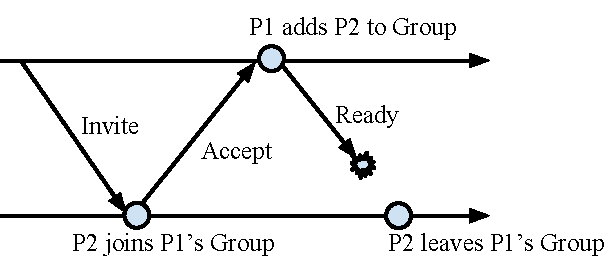
\includegraphics[width=\linewidth]{LostReady.pdf}
\caption{The grouping processes effects the outcome of elections} \label{fig:lostready}
\end{figure}

Without the ready acknowledgment message, the probability a member remains in a group in the first round after an election has a different probability than each subsequent round.
By adding the extra message, the observation of the coordinator must be the state of the member of the group.
As a consequence, the probability a member remains in a group in the first round after an election is identical to each subsequent round.

\subsection{Failure Detection}

Members cannot leave a group without the leader's permission.
Members do not suspect the coordinator has failed, only the coordinator may suspect the members.
This change is shown in Figure \ref{fig:statemachine2}, denoted by the elements marked with an asterisk.
For the purpose of starting an election, an ``Are You There'' message and its negative response are considered equivalent to a ``Are You Coordinator'' message and a positive response.
On receipt of the negative response, the member will immediately recover and become a leader.
This assumption relies on ``Are You Coordinator'' and ``Are You There'' messages being sent at roughly the same time.
This change leads to a live-lock situation in a crash failure, where the group's leader crashes and does not return and as a consequence the remaining members are trapped in a group without a leader.
For the purpose of this work, we have disregarded these live lock scenarios.


\subsection{Creation of A Profile Chain}

The election algorithm produces and distributes a set of processes $UpPeers$ and a coordinator of that set.
$UpPeers$ is distributed via message passing and maintained by the coordinator.
Different processes may have different versions of $UpPeers$ for a given coordinator as processes enter and leave the group.
However, a process will eventually receive an up-to-date version of $UpPeers$ from the coordinator, or it will leave the group.

To model the behavior of the algorithm, at each time-step the selected process recorded the cardinality of its membership set $UpPeers$.
The selected process was always the coordinator of any formed group, and was the only process that could lead a multi-process group.
The cardinality of $UpPeers$ directly mapped to the state in the Markov Chain.
For example given the membership set $S=\{P1,P2,P3\}$, then $\left | S \right |=3$ and the state of the system in the Markov chain is also $i=3$.

The profile Markov chain for the algorithm was constructed as a closed form representation of the algorithm's behavior.
Each round, the behavior is described by two components: maintaining a group and inviting other processes into the group.
The coordinator will exchange a ``Are You Coordinator'' message and the peer will respond to verify is still available.
To maintain a group of $m$ other processes, the probability is defined as a random variable with the following probability distribution (pdf):

\begin{equation}
 \Pr_{M}(X=k; m) =
   \begin{cases}
    \binom{m}{k} p^{2k}(1-p^2)^{m-k}, & \text{if } 0 \leq k \leq m \\
    0,                                & \text{otherwise} \\
  \end{cases}
\end{equation}

Where $k$ is the number of processes remaining in a group selected from $m$ processes.
A process will leave a group if, from the considered process's perspective, they do not respond to an ``Are You Coordinator'' message.
Members cannot change their state without coordinating with the leader.

To invite other processes to the group, the two processes ultimately exchange up to 8 messages.
In a round, a single process can invite many other processes to its group.
From a selection of $n$ other coordinators, the probability distribution for joining a new group with $k$ of the $n$ processes is:

\begin{equation}
	\Pr_{I}(Y=k; n) =
	\begin{cases}
		\binom{n}{k} p^{8k}(1-p^8)^{n-k}, & \text{if } 0 \leq k \leq n \\
		0,                                & \text{otherwise} \\
	\end{cases}
\end{equation}

In the profile chain, in a state $s$ that describes the number of processes in a group, the probability of transitioning from $s$ to $s'$ with $n$ total processes (including the considered process) is:

\begin{align} \Pr_{T}(Z=s'; n; s) = \sum_{i=0}^{s-1} &\Pr_{M}(X=i; s-1) \cdot
\nonumber \\ &\Pr_{I}(X=s'-i; n-s-1) \end{align}

From this distribution, a set of transition probabilities can be calculated for a given omission rate $p$ and number of processes $n$.
This set of transition probabilities forms a profile Markov chain $P$, which can be evaluated to for any number of processes $n$ and omission rate $p$.
The generated profile chain is ergodic when $0<p<1.0$. The profile chain is a stationary Markov chain.
